%%%%%%%%%%%%%%%%%%%%%%%%%%%%%%%%%%%%%%%%%
% Beamer Presentation
% LaTeX Template
% Version 1.0 (10/11/12)
%
% This template has been downloaded from:
% http://www.LaTeXTemplates.com
%
% License:
% CC BY-NC-SA 3.0 (http://creativecommons.org/licenses/by-nc-sa/3.0/)
%
%%%%%%%%%%%%%%%%%%%%%%%%%%%%%%%%%%%%%%%%%

%----------------------------------------------------------------------------------------
%	PACKAGES AND THEMES
%----------------------------------------------------------------------------------------

\documentclass{beamer}
\usepackage{xeCJK}
\usepackage{times}
\usepackage{multirow}
\usepackage{diagbox}
\usepackage{subfigure}
\usepackage{graphicx}
\usepackage{booktabs}
\usepackage{float}
\usepackage{algorithm}
\usepackage{algorithmic}
%\usepackage{caption}

\floatname{algorithm}{算法}  
\renewcommand{\algorithmicrequire}{\textbf{初始化:}}  
\renewcommand{\algorithmicensure}{\textbf{直到收敛,返回}}
%\renewcommand{\algorithmicrepeat}{\textbf{迭代,根据以下步骤更新:}}
\newcommand{\INDSTATE}[1][1]{\STATE\hspace{#1\algorithmicindent}}
\DeclareMathOperator*{\argmax}{arg\,max}
%\captionsetup[subfigure]{labelformat=empty}
\setbeamertemplate{caption}[default]
\setbeamertemplate{section in toc}[circle]

\newcommand{\cccve}{CCC\{$v_\mathrm{e}$\}}
\newcommand{\ccckt}{CCC\{$K^\mathrm{trans}$\}}
\newcommand{\kt}{$K^\mathrm{trans}$}
\newcommand{\Ve}{$v_\mathrm{e}$}
\newcommand{\argmin}{\operatornamewithlimits{arg\ min~}}

%\setCJKfamilyfont{song}{SimSun}                             %宋体 song
%\newcommand{\song}{\CJKfamily{song}} 

\usefonttheme{serif}
\usepackage{fourier}
\mode<presentation> {

% The Beamer class comes with a number of default slide themes
% which change the colors and layouts of slides. Below this is a list
% of all the themes, uncomment each in turn to see what they look like.

%\usetheme{default}
%\usetheme{AnnArbor}
%\usetheme{Antibes}
%\usetheme{Bergen}
%\usetheme{Berkeley}
%\usetheme{Berlin}
%\usetheme{Boadilla}
%\usetheme{CambridgeUS}
%\usetheme{Copenhagen}
%\usetheme{Darmstadt}
%\usetheme{Dresden}
%\usetheme{Frankfurt}
%\usetheme{Goettingen}
%\usetheme{Hannover}
%\usetheme{Ilmenau}
%\usetheme{JuanLesPins}
%\usetheme{Luebeck}
%\usetheme{Madrid}
\usetheme{Malmoe}
%\usetheme{Marburg}
%\usetheme{Montpellier}
%\usetheme{PaloAlto}
%\usetheme{Pittsburgh}
%\usetheme{Rochester}
%\usetheme{Singapore}
%\usetheme{Szeged}
%\usetheme{Warsaw}

% As well as themes, the Beamer class has a number of color themes
% for any slide theme. Uncomment each of these in turn to see how it
% changes the colors of your current slide theme.

%\usecolortheme{albatross}
%\usecolortheme{beaver}
%\usecolortheme{beetle}
%\usecolortheme{crane}
%\usecolortheme{dolphin}
%\usecolortheme{dove}
%\usecolortheme{fly}
%\usecolortheme{lily}
%\usecolortheme{orchid}
%\usecolortheme{rose}
%\usecolortheme{seagull}
%\usecolortheme{seahorse}
%\usecolortheme{whale}
%\usecolortheme{wolverine}

%\setbeamertemplate{footline} % To remove the footer line in all slides uncomment this line
%\setbeamertemplate{footline}[page number] % To replace the footer line in all slides with a simple slide count uncomment this line

%\setbeamertemplate{navigation symbols}{} % To remove the navigation symbols from the bottom of all slides uncomment this line
}

%\usepackage{graphicx} % Allows including images
 % Allows the use of \toprule, \midrule and \bottomrule in tables

%----------------------------------------------------------------------------------------
%	TITLE PAGE
%----------------------------------------------------------------------------------------

\title[博士学位论文答辩]{南京理工大学\\博士学位论文答辩模板}

\author[南京理工大学]{
答辩人:张三 \\
导师:李四\quad 教授
} % Your name
\institute[南京理工大学] % Your institution as it will appear on the bottom of every slide, may be shorthand to save space
{
南京理工大学 \\ % Your institution for the title page
\medskip
**学院 
}
\date{****年**月**日} % Date, can be changed to a custom date

\begin{document}

\begin{frame}
\titlepage % Print the title page as the first slide
\end{frame}

\begin{frame}
\frametitle{目录}
\scalebox{0.8}{
\begin{minipage}{1\linewidth}
     \tableofcontents
     \end{minipage}}
 \end{frame}

%----------------------------------------------------------------------------------------
%	PRESENTATION SLIDES
%----------------------------------------------------------------------------------------

%------------------------------------------------
\section{引言}
%------------------------------------------------
%\AtBeginSection[]
%{
    \begin{frame}
        \tableofcontents[currentsection,hideallsubsections]
    \end{frame}
%}

\subsection{研究背景}


\subsection{论文研究动机和研究成果}
\begin{frame}
\textbf{研究动机:}

\textbf{研究成果:}
\end{frame}

%------------------------------------------------
\section{第一部分}
%------------------------------------------------
%\AtBeginSection[]
%{
    \begin{frame}
        \tableofcontents[currentsection,hideallsubsections]
    \end{frame}
%}


\begin{frame}
	\frametitle{基于二阶时空TGV和核范数的模型}
针对动态MR图像,基于图像分解的思想,利用二阶时空TGV和核范数,提出模型:
\begin{equation}
\min_{L,S} \frac{1}{2}\|A(L+S)-B\|_{\mathrm{F}}^2+\mathrm{TGV}^2_\alpha(S)+\beta\|L\|_*.
\label{propopsed}
\end{equation}
\end{frame}


\begin{frame}
%	\frametitle{模型的求解}
	\begin{center}
	\scalebox{0.95}{
	\begin{minipage}{1\linewidth}
	\begin{algorithm}[H]
	\caption{二阶时空TGV和低秩分解模型的Primal-Dual算法}
	\label{alg:proposed}
	\begin{algorithmic}
		\REQUIRE $\sigma$, $\tau$, $S_0$, $L_0$,令 $L_0=A^*B$,$S_0=0$;
		\INDSTATE[-1] \textbf{迭代:根据以下步骤更新参数:}	
		\STATE 1. $p^{n+1} = \mathcal{P}_{\alpha_1}(p^n+\sigma(\nabla \bar{S}^n-\bar{w}^n))$;
		\STATE 2. $q^{n+1} = \mathcal{P}_{\alpha_0}(q^n+\sigma\mathcal{E}(\bar{w}^n))$;
		\STATE 3. $\lambda^{n+1} = (\lambda^{n}+\sigma(A(\bar{L}^n+\bar{S}^n)-B))/(1+\sigma)$;
		\STATE 4. $S^{n+1} = S^n-\tau(A^*\lambda^{n+1}-\mathrm{div}_1 p^{n+1})$;
		\STATE 5. $w^{n+1} = w^n+\tau(\mathrm{div}_2q^{n+1}+p^{n+1})$;
		\STATE 6. $L^{n+1} = \mathcal{S}_\beta(L^n-\tau A^*r^{n+1})$;
		\STATE 7. $\bar{S}^{n+1} = 2S^{n+1}-S^n$;
		\STATE 8. $\bar{w}^{n+1} = 2w^{n+1}-w^n$;
		\STATE 9. $\bar{L}^{n+1} = 2L^{n+1}-L^n$;
		\ENSURE $x^{n+1}$
	\end{algorithmic}
\end{algorithm}
\end{minipage}}
\end{center}
\end{frame}


%------------------------------------------------
\subsection{数值实验结果与分析}


\begin{frame}
	\frametitle{数值实验结果}
%	\begin{center}
	\scalebox{0.8}{
	\begin{minipage}{1\linewidth}
\begin{table}
	\centering
	\caption{各个模型在不同数据上的重建结果(伪径向采样)}
	\begin{tabular}{|c|c|c|c|c|c|c|}
		\hline
		\hline
		\multicolumn{2}{|c|}{\diagbox{模型}{数据集}}& 躯干体模 & 心脏灌注 & 胸部1 & 胸部2 & 胸部3\\	
		\hline
		\multirow{2}{*}{Zerofilled}
		&SER & 20.54 & 14.80 & 11.32 & 11.57 & 14.85\\
		\cline{2-7}&SSIM & 0.8321 & 0.8855 & 0.4820 & 0.5897 & 0.7086\\
		\hline
		\multirow{2}{*}{kt-SLR}
		&SER & \textbf{33.35} & 17.58 & 17.42 & 13.61 & 18.38\\
		\cline{2-7}&SSIM & 0.9880 & 0.9412 & 0.7712 & 0.6956 & 0.8461\\
		\hline
		\multirow{2}{*}{kt-RPCA}
		&SER & 29.27 & 18.33 & 19.31 & 14.82 & 19.81\\
		\cline{2-7}&SSIM & 0.9700 & 0.9447 & 0.8857 & 0.7920 & 0.9068\\
		\hline
		\multirow{2}{*}{L+S}
		&SER & 27.99 & 19.12 & 17.60 & 14.74 & 19.91\\
		\cline{2-7}&SSIM & 0.9514 & 0.9490 & 0.7675 & 0.7319 & 0.8791\\
		\hline
		\multirow{2}{*}{ICTGV}
		&SER & 26.88 & 17.87 & 16.31 & 12.18 & 16.84\\
		\cline{2-7}&SSIM & 0.9435 & 0.9405 & 0.6735 & 0.6080 & 0.7693\\
		\hline
		\multirow{2}{*}{Proposed}
		&SER & 32.74 & \textbf{19.57} & \textbf{20.56} & \textbf{16.24} & \textbf{21.08}\\
		\cline{2-7}&SSIM & \textbf{0.9917} & \textbf{0.9514} & \textbf{0.9402} & \textbf{0.9091} & \textbf{0.9356}\\
		\hline
	\end{tabular}
	\label{tab:result3}
\end{table}
\end{minipage}}
%\end{center}
\end{frame}

\begin{frame}
\hspace{-0.7cm}
\begin{minipage}{1\textwidth}
%	\begin{figure}[htbp]
	\centering
		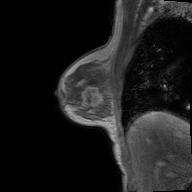
\includegraphics[width=0.5\textwidth]{breast.png}
%	\caption{各个模型在躯干体模数据上的重建结果(第1帧)}
%\end{figure}
\end{minipage}
\end{frame}

%------------------------------------------------
\section{第二部分}
%------------------------------------------------
%\AtBeginSection[]
%{
    \begin{frame}
        \tableofcontents[currentsection,hideallsubsections]
    \end{frame}
%}

\begin{frame}
	
\end{frame}

%------------------------------------------------
\section{第三部分}
%------------------------------------------------
%\AtBeginSection[]
%{
    \begin{frame}
        \tableofcontents[currentsection,hideallsubsections]
    \end{frame}
%}

\begin{frame}
	
\end{frame}
%------------------------------------------------
\section{全文总结}

\begin{frame}
    \tableofcontents[currentsection,hideallsubsections]
\end{frame}

\begin{frame}
	
\end{frame}


%------------------------------------------------

\begin{frame}
\centerline{感谢各位专家、老师来参加我的博士论文学位答辩!}
\end{frame}

%----------------------------------------------------------------------------------------
\end{document}